% To familiarize yourself with this template, the body contains
% some examples of its use.  Look them over.  Then you can
% run LaTeX on this file.  After you have LaTeXed this file then
% you can look over the result either by printing it out with
% dvips or using xdvi.
%

\documentclass[twoside]{article}
%\usepackage{soul}
\usepackage{./lecnotes_macros}


\begin{document}
%FILL IN THE RIGHT INFO.
%\lecture{**LECTURE-NUMBER**}{**DATE**}{**LECTURERS**}{**SCRIBE**}
\lecture{21}{14 January 2025}{Maria Francis and M. V. Panduranga Rao}{Gautam Singh}
%\footnotetext{These notes are partially based on those of Nigel Mansell.}

%All figures are to be placed in a separate folder named ``images''

% **** YOUR NOTES GO HERE:

\section{Differential Cryptanalysis}
In differential cryptanalysis, we exploit the XOR between plaintext pairs in a chosen plaintext attack to find the secret key bits used in the cryptosystem. Per DES round, the XOR of a pair of inputs remains invariant.

\begin{enumerate}
    \item Expansion \(E\) to get \(Si_E\).
    \item XOR with subkey \(K\) to get \(Si_I = Si_E \oplus Si_K\).
    \item Permutation after S boxes to get \(Si_O\).
\end{enumerate}

\begin{figure}[!ht]
    \centering
    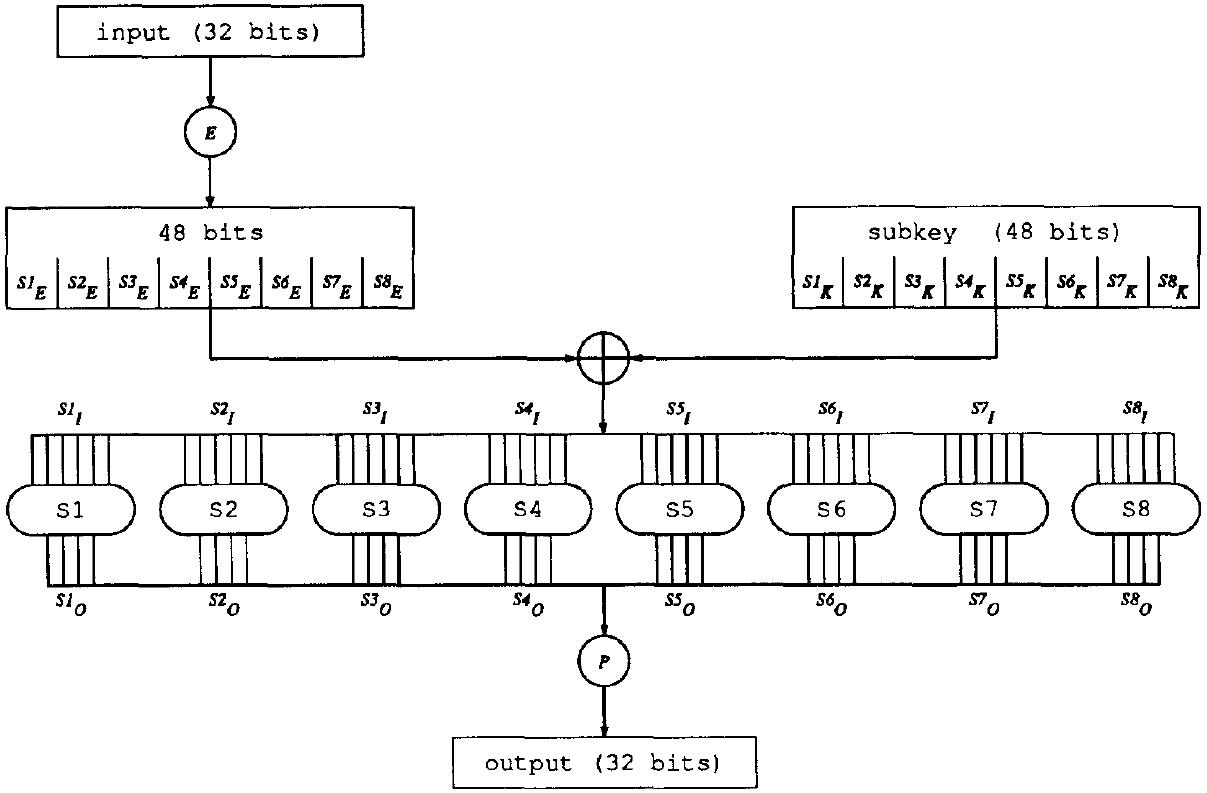
\includegraphics[width=0.5\linewidth]{images/des_f.png}
    \caption{The \(F\) function of DES}
    \label{fig:des-f}
\end{figure}

The authors want to carry out a probabilistic analysis on the S boxes; this will estimate the number of plaintexts to be used for cryptanalysis. Immediately, they abstract out the key schedule by assuming all round subkeys are independent of each other.

\subsection{Probability Analysis of S Boxes}
We now focus on the S boxes. Suppose \(Si_I^\prime = Si_I \oplus Si_I^*\) is the input XOR and \(Si_O^\prime = Si_O \oplus Si_O^*\) is the output XOR. The authors compute the joint probability distribution function (PDF) of the input-output XOR pair \((Si_I^\prime, Si_O^\prime)\). This results in a 64-by-16 table of frequency distributions, since S boxes take 6-bit inputs to 4-bit outputs. This is called the \emph{pairs XOR distribution table}.

For cryptanalysis, we can now talk about the conditional probability \(\Pr(Si_I^\prime \mid Si_O^\prime)\). At each round of DES, we know \(Si_I^\prime = Si_E^\prime\) and we observe \(Si_O^\prime\). Using the pairs XOR distribution of that S box, we can get more information about \(Si_I\) and \(Si_I^*\), which can then be used to compute \(Si_K = Si_I \oplus Si_E = Si_I^* \oplus Si_E^*\). It is trivial to now extend this pairs XOR probability to the entire \(F\)-function used in the Feistel network, since the only nonlinearlity in the input XOR is provided by the S boxes.

Suppose \(Si_I^\prime \rightarrow Si_O^\prime\) with probability \(p_i\) by the S box \(Si\). Then, \(S_I\prime \rightarrow S_O^\prime\) with probability \(P = \prod_{i=1}^8p_i\) by the F function of that particular round. That is, the probabilities are \emph{multiplicative}. Further, the \(P_j\)'s across the rounds \(j\) will also multiply, thereby reducing the chances of a particular input-output XOR pair of the entire iterated cryptosystem. The aim is to keep the total \(P = \prod_{i=1}^nP_i\) over the \(n\) rounds of this cryptosystem high enough to be able to perform cryptanalysis quickly.

\subsection{Characteristic}

To formalize the cryptanalysis of iterated cryptosystems, we are introduced to the notion of a \emph{characteristic}. This is a tuple \(\Omega = (\Omega_P, \Omega_\Lambda, \Omega_T)\) which characterizes the XOR of a pair of plaintexts as they go through the same cryptosystem. The authors write \(\Omega_\Lambda = (\Lambda_1, \ldots, \Lambda_n)\) such that \(\Lambda_i = (\lambda_I^i, \lambda_O^i)\) where \(\lambda_I^i\) is the input to the \(F\) function in the \(i\)-th round and \(\lambda_O^i\) is the corresponding output. For intermediate rounds, we have

\begin{equation}
    \lambda_O^i = \lambda_I^{i+1} \oplus \lambda_I^{i-1}.
    \label{eq:lambda-io-rel}
\end{equation}

\begin{figure}[!ht]
    \centering
    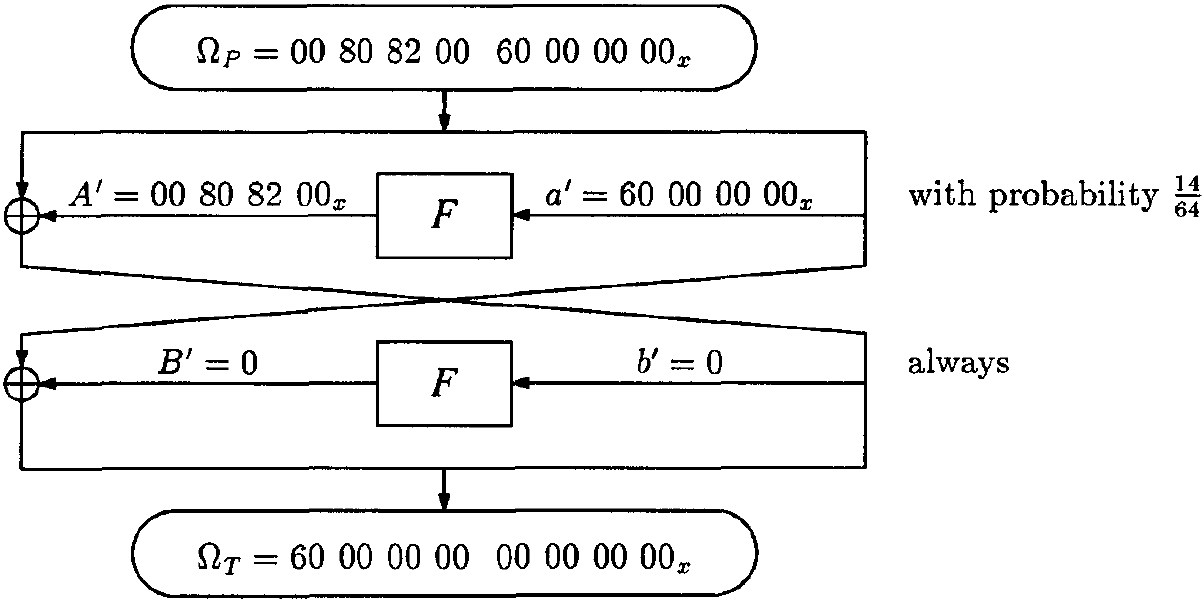
\includegraphics[width=0.5\linewidth]{images/des_char.png}
    \caption{An example of an \(n=2\) round characteristic.}
    \label{fig:des-char}
\end{figure}

Call a pair of plaintexts \emph{right} with respect to \(\Omega\) and an independent key \(K\) if this pair generates the XORs using the key \(K\) over the \(n\) rounds of encryption, and \emph{wrong} otherwise. The probability of a characteristic is then the fraction of such plaintext pairs which satisfy \(P^\prime = \Omega_P\). It is not hard to see that they can be concatenated and the probabilities are multiplicative.

When \(\Omega_T\) is the swapped value of the halves of \(\Omega_P\), we get an iterative characteristic: one that we can concatenate with itself to get characteristics of arbitrary length. An example of an iterative characteristic is shown in \autoref{fig:des-iter-char}.

\begin{figure}[!ht]
    \centering
    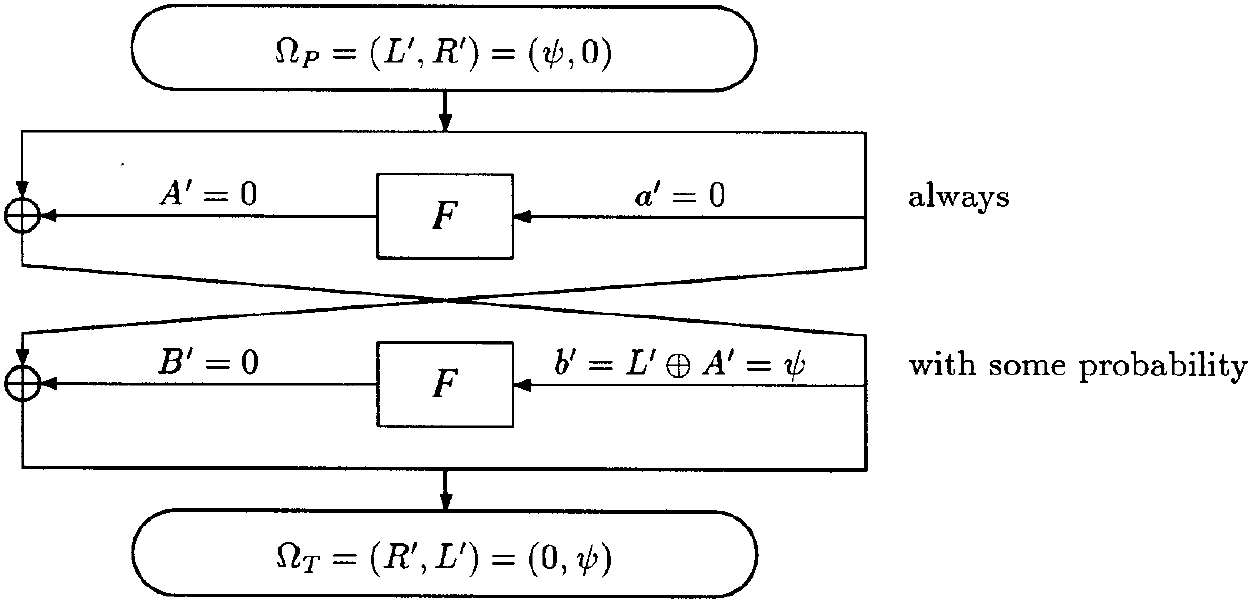
\includegraphics[width=0.5\linewidth]{images/des_iter_char.png}
    \caption{Example of an iterative characteristic where \(\psi \rightarrow 0\).}
    \label{fig:des-iter-char}
\end{figure}

\subsection{Signal-to-Noise Ratio}
With the knowledge of characteristics and their probabilities, we need to analyze a large enough number of plaintext pairs and find some bits of a subkey (and thus the master key) entering certain S boxes. This is done with a simple counting approach, and intuitively the most frequently suggested subkey is likely to be the actual subkey used.

However, we did not account for the time and memory complexity of such counting approaches. To do this, we define the \emph{signal-to-noise ratio} of a counting scheme as the ratio of the number of right pairs to the average count, denoted by \(S/N\). Suppose we want to find \(k\) subkey bits in a cryptosystem of block size \(m\). Let \(\alpha\) be the average count per counted pair and \(\beta\) be the fraction of counted pairs. Then, for a characteristic probability \(p\),

\begin{equation}
    S/N = \frac{mp}{\frac{m\alpha\beta}{2^k}} = \frac{2^kp}{\alpha\beta}.
\end{equation}

This shows that \(S/N\) is independent of the block size and the number of pairs used. A larger \(S/N\) implies fewer plaintext pairs are needed and conversely. To improve \(S/N\), we consider fewer plaintexts that can pair up to form right pairs for various characteristics such as \emph{quartet} (four plaintexts with two pairs each of two characteristics) and \emph{octet} (eight plaintexts, four pairs each of three characteristics). This also saves memory since we can reuse the plaintexts for different characteristics.

\end{document}
